\documentclass[12pt]{standalone}
\usepackage{tikz}
\begin{document}
  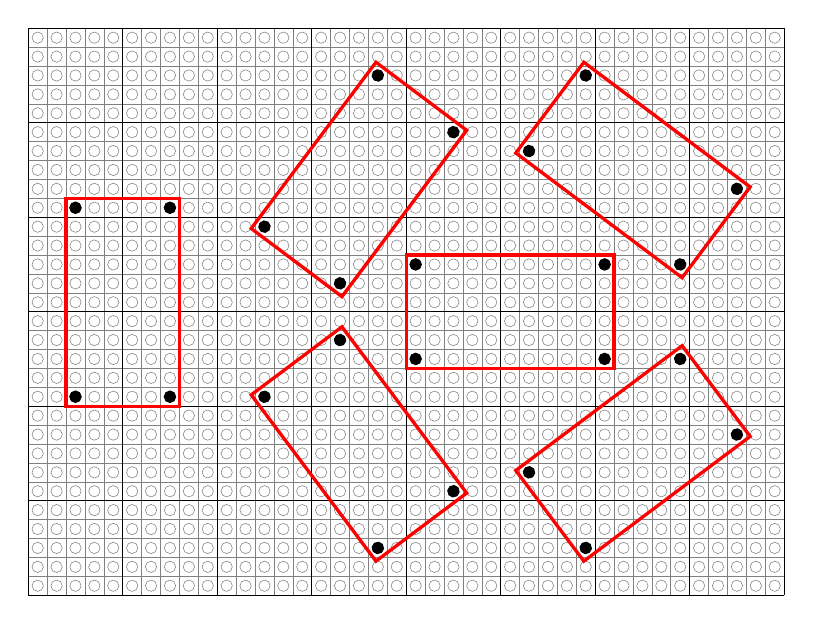
\begin{tikzpicture}[scale=0.24]
    \draw[style=help lines] (0,0) grid (40,30);
    \draw (0,0) grid[step=5] (40,30);
    \foreach \x in {0,...,39}{
      \foreach \y in {0,...,29}{
        \draw[style=help lines] (\x+0.5,\y+0.5) circle (0.3);
      }
    }
    \foreach \a/\b in {
      (5,15.5)/0,
      (25.5,15)/90,
      (17.5,22)/143.1301,
      (32,22.5)/53.1301,
      (17.5,8)/-143.1301,
      (32,7.5)/-53.1301
    }{
      \begin{scope}[shift={(\a)},rotate={\b}]
        \draw[red,very thick] (-3,-5.5) -- (3,-5.5) -- (3,5.5) -- (-3,5.5) -- cycle;
        \foreach \p in {(-2.5,-5),(2.5,-5),(2.5,5),(-2.5,5)}{
          \draw[fill=black] \p circle (0.3);
        }
      \end{scope}
    }
  \end{tikzpicture}
\end{document}
